\documentclass[a4paper, twoside, 11pt, openright]{article}
\usepackage[utf8]{inputenc}
\usepackage{polski}
\usepackage{float}
\usepackage[T1]{fontenc}
\usepackage{url}

\raggedbottom

\usepackage[left=3.0cm, right=2.0cm, top=2.5cm, bottom=2.5cm]{geometry}

% PERSONAL data about the thesis
\newcommand{\myTitle}{Metodyka porównania algorytmów prognozy do wspomagania decyzji giełdowych}
\newcommand{\myName}{Nikodem Wiśniewski}
\newcommand{\myNumber}{260907}
\newcommand{\myThesisType}{Praca dyplomowa magisterska}
\newcommand{\myCourse}{Informatyka}
\newcommand{\myProf}{dr hab. inż. Jerzy Balicki}
\newcommand{\myFaculty}{Wydział Matematyki i Nauk Informacyjnych}
\newcommand{\myUni}{Politechnika Warszawska}
\newcommand{\myLocation}{Warszawa}
\newcommand{\myYear}{2019}
\newcommand{\myKeywords}{}
\newcommand{\myKeywordsPL}{}



% DOCUMENT settings


\usepackage{graphicx}
\usepackage{multirow}
\usepackage{indentfirst}
\usepackage{wrapfig}
\usepackage[font=footnotesize, % equivalent to 9 pt font
			labelfont=bf, 
			justification=justified, 
			singlelinecheck=false]{caption} 
%\usepackage[justification=centering]{subcaption} % two images side by side captions
\usepackage{tabularx, booktabs} % pretty LaTeX tables
\usepackage{siunitx} % units SI e.g. \SI{10}{\kilogram\per\meter\square}
\usepackage{mathtools} % amsmath, symbols such as brackets, arrows, equation numbering only for referrenced eqs.
%\usepackage[parfill]{parskip} % spacing between paragraphs instead of indent
%\parfillskip 0pt plus 0.75\textwidth % get rid of widows at the end of paragraphs
\frenchspacing % for "Polish" spaces after the sentence
\usepackage{polski} % Polish rules of hyphenation
\usepackage{dashrule} % for dotted lines in declarations page
\usepackage{emptypage} % removes headers on empty pages
\usepackage{fancyhdr} % header and footer settings
\usepackage{subfigure}

\pagestyle{fancy}
\fancyhf{}
\newcommand{\fncyfront}{%
	\fancyhead[RO]{}
	\fancyfoot[RO]{}
	\fancyhead[LE]{}
	\fancyfoot[LE]{}
	\fancyhead[RE,LO]{}
	\fancyfoot[C]{}
	\renewcommand{\headrulewidth}{0pt}}
\newcommand{\fncymain}{%
	\fancyhead[RO]{{\footnotesize \rightmark}}
	\fancyfoot[RO]{\thepage}
	\fancyhead[LE]{{\footnotesize \leftmark}}
	\fancyfoot[LE]{\thepage}
	\fancyfoot[C]{}
	\renewcommand{\headrulewidth}{0.3pt}}
	
\renewcommand*{\tablename}{Tabela} 
	
\newcolumntype{P}[1]{>{\centering\arraybackslash}p{#1}}
\newcolumntype{M}[1]{>{\centering\arraybackslash}m{#1}}



% FONT settings
\usepackage[T1]{fontenc}
\usepackage{uarial} % you can change to 'helvet' for Helvetica clone, 'uarial' for Arial clone, 'lmodern' for Latin Modern
%\renewcommand{\familydefault}{\sfdefault} % change font to sans serif
\usepackage{amsfonts} % mathematical fonts
\usepackage{inconsolata} % monospaced font in urls and \texttt
%\usepackage{url}
%\urlstyle{same}

% DEBUG
\usepackage{lipsum}
\usepackage{etoolbox} % removes page number in table of contents
\patchcmd{\chapter}{plain}{empty}{}{}


\begin{document}
\fncyfront
%*******************************************************
% Titlepage
%*******************************************************
\begin{titlepage}
\begingroup
\begin{center}		
			
\includegraphics[width=1.0\textwidth]{img/pw_header}
			
			\vspace{1.0cm}
			\fontsize{24}{30}\selectfont\myThesisType
			\fontsize{12}{14}\selectfont
			
			\vspace{0.5cm}
			na kierunku \myCourse \\
			\vspace{1cm}
			{\fontsize{14}{18}\selectfont \myTitle} \\ 
			
			\vspace{1.5cm}
			\fontsize{21}{25}\selectfont \myName \\
			\fontsize{12}{14}\selectfont
			Numer albumu \myNumber \\

			\vspace{6.5cm}
			promotor \\
			\myProf \\
			\vspace{0.5cm}
			\vfill 
			Warszawa, \myYear
        \vfill                      
\end{center}
\endgroup
\end{titlepage}

\newpage
\hfill
\begin{table}[b]
\centering
\begin{tabular}[t]{ccc}
............................................. & \hspace*{100pt} & .............................................\\
podpis promotora & \hspace*{100pt} & podpis autora
\end{tabular}
\end{table}

\fncymain

\newpage

\tableofcontents

\newpage

\section{Opis pracy}

Celem tej pracy było opracowanie, ocena i porównanie różnych modeli predykcji cen akcji na giełdzie papierów wartościowych lub innych alternatywnych giełdach np. giełda kryptowalut.

\subsection{Giełda}

Giełda z definicji jest miejscem wymiany towarów przez sprzedawców i kupców. Giełdy można podzielić na giełdy towarowe, pieniężne lub usługowe. Wymiany na tradycyjnych giełdach przebiegają przede wszystkim podczas sesji, które są organizowane w określonych dniach i godzinach. Najpopularniejszym rodzajem giełd są giełdy pieniężne, a w szczególności giełdy papierów wartościowych. Największymi giełdami papierów wartościowych są \textit{NYSE (New York Stock Exchange)}\cite{nyse}, \textit{NASDAQ}\cite{nasdaq} oraz \textit{JPX (Japan Exchange Group)}\cite{jpx}. Na każdej z tych giełd w dniach, w których prowadzone są sesje, dochodzi do transakcji opiewających na łączną kwotę rzędu miliardów dolarów amerykańskich.

\bigskip

 Jednym z wymienianych na giełdzie towarów są akcje różnorodnych spółek. Każda spółka, która jest obecna na giełdzie ma przypisany symbol giełdowy (\textit{ticker}). Symbol giełdowy jest skrótowym kodem do identyfikowania spółek na określonej giełdzie (przykładowe symbole: \textit{GOOGL}, \textit{MSFT}, \textit{AMZN}). Podczas każdej sesji dokonywane są transakcje milionów akcji, których cena regulowana jest jedynie przez wolny rynek. Wynikiem tego jest duża zmienność cen akcji, spowodowana różnymi spekulacjami lub upublicznianiem informacji o konkretnej spółce.


\subsection{Dostępne dane}

Przed przystąpieniem do wyboru metod należy zastanowić się nad danymi wejściowymi do algorytmów przewidujących. Podstawowe dane dostępne na giełdzie to:
\begin{itemize}
\item{Data}
\item{Cena zamknięcia} cena akcji pod koniec dnia
\item{Cena otwarcia} cena akcji na początku dnia
\item{Ilość akcji w obrocie danego dnia}
\item{Najniższa cena akcji danego dnia}
\item{Najwyższa cena akcji danego dnia}
\end{itemize}

 Przy korzystaniu z wartości cen akcji należy również uwzględnić podział akcji(tak zwany \textit{split}). Gdy jakaś spółka decyduje się na podział swoich akcji oznacza to, że każda z akcji dzieli się na dwie akcje o cenie wynoszącej połowę pierwotnej ceny. Taki zabieg pozwala na zmniejszenie ceny pojedynczej akcji dzięki czemu może stać się ona dostępna dla większej ilości inwestorów. 

\subsection{Źródło danych}

Ze względu na małą dostępność gotowych danych do trenowania modeli predykcyjnych w pracy zostało wykorzystane darmowe źródło danych giełdowych \textit{Alpha Vantage} \cite{alphavantage}. Jest to API pozwalające na pobranie danych historycznych dla konkretnej spółki poprzez podanie symbolu giełdowego. Do pobrania danych została wykorzystana lista symboli z giełdy NASDAQ \cite{nasdaq}. Spośród wszystkich spółek zostały odrzucone te, których historia giełdowa była niepełna, zaburzona lub miała mniej niż 3000 dni giełdowych. Pozwoliło to na wyselekcjonowanie zbioru ponad 900 spółek na podstawie których trenowane i testowane były wybrane modele. Wszystkie dane po pobraniu zostały zapisane w lokalnej bazie \textit{MongoDB} \cite{mongodb} w celu trwałego przechowania danych i optymalizacji w ich pobieraniu do pamięci.

\subsection{Predykcja}

Na rysunku \ref{alphabet_history} widoczne są zmiany cen akcji spółki \textit{Alphabet Inc.} w latach 2004-2018. Analizując ten wykres można z łatwością wskazać daty, w których opłacalnym było zainwestowanie w akcje, a następnie je sprzedać by osiągnąć zysk. Niestety stwierdzenie czy wartość akcji w przyszłości spadnie, czy wzrośnie, nie jest tak trywialne jak odczytywanie danych historycznych. Przewidywanie przyszłych cen akcji jest głównym zajęciem zarówno inwestorów indywidualnych jak i instytucjonalnych. Skuteczne odgadywanie przyszłych wzrostów lub spadków cen pozwoliłoby na osiąganie ponadprzeciętnych zysków i unikanie strat.


\begin{figure}[H]
\centering 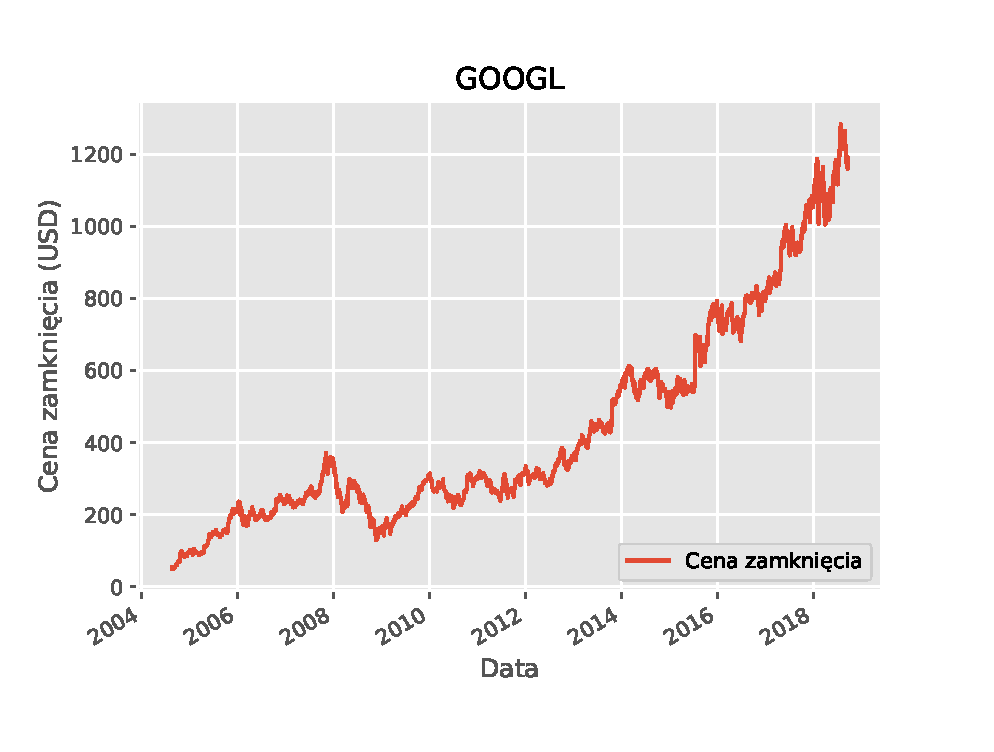
\includegraphics[scale=0.9]{img/linear_regression/l_r_stock_data}
\caption{Wykres cen akcji spółki \textit{Alphabet Inc}}
\label{alphabet_history}
\end{figure}

\subsubsection{Przewidywany parametr}

Najbardziej pożytecznym parametrem akcji, którego przewidywanie daje inwestorowi największe szanse na zysk jest \textit{cena zamknięcia}. Znajomość ceny zamknięcia z kolejnego dnia daje możliwość podjęcia skutecznych decyzji inwestycyjnych. Przykładem parametru, który byłby bez wartości jest ilość akcji w obrocie w przyszłości, ta liczba sama w sobie nie niesie informacji o spadku lub wzroście cen. Do tematu prognozowania można podejść na dwa sposoby:
\begin{itemize}
\item{\textbf{dokładny}, przewidywanie konkretnych wartości akcji}
\item{\textbf{dyskretny}, predykcja wzrostu, spadku lub utrzymania ceny}
\end{itemize}

\subsubsection{Hipoteza błądzenia losowego}

Zgodnie z hipotezą błądzenia losowego \cite{randwalk}, krótkoterminowo, ceny akcji zmieniają się według nieprzewidywalnych schematów. Zmiany minutowe cen akcji są więc dużo cięższe do przewidzenia niż zmiany dobowe. Z tego względu przewidywanie wartości w okresie krótszym niż jedna doba, nie zostało uwzględnione w obszarze badań tej pracy.

\subsection{Metodyka tworzenia modeli}

Ponieważ zagadnienie przewidywania giełdy jest nietrywialne ze względu na losowe wahania wpływające na ceny akcji, do stworzenia każdego z modeli do predykcji, należy rozważyć wykorzystanie zróżnicowanych założeń:
	
\begin{itemize}
\item{\textbf{Prognozowanie dokładne/dyskretne} }
\item{\textbf{Liczba dni}, z których prognozowana jest wartość.}
\item{\textbf{Dobór danych pobranych z giełdy}, selekcja wartości wejściowych}
\item{\textbf{Dobór spółek uczących i testujących}}
\end{itemize}

\subsubsection{Prognozowanie - regresja czy klasyfikacja?}

Potencjalnie korzystniejszym podejściem jest przewidywanie dokładnych cen akcji, gdyż pozwoli na dokładniejsze aproksymowanie ceny. Jednak w celu skutecznej oceny modelu, który ma służyć do celów inwestycyjnych, zamiast przewidywania dokładnej ceny zamknięcia należy przewidywać wzrosty oraz spadki ceny. Binarne przewidywanie z dnia na dzień może jednak okazać się nieprzydatne ze względu na to jak przebiega obrót akcjami. Akcje kupuje i sprzedaje się za pomocą domu maklerskiego, który pobiera prowizje za każdą transakcję. Obecnie najniższe prowizje na polskim rynku są na poziomie $0,19\%$ za transakcję. Pojedyncza operacja dająca zarobić na przewidzianej cenie wymaga kupienia, a następnie sprzedania akcji, wobec czego łączna prowizja wyniesie przy zaokrągleniu $0,4\%$. Wszystkie wahania cen poniżej tej wartości są teoretycznie bez znaczenia dla inwestora. W związku z powyższym wnioskowaniem należy zastosować model, który przewiduje trzy wartości:
\begin{itemize}
\item spadek ceny poniżej $0,4\%$
\item wzrost ceny powyżej $0,4\%$
\item utrzymanie zmiany ceny w przedziale $(-0,4; 0,4)\%$
\end{itemize}


Na rysunku \ref{l_r_pct_change_last_30} można zaobserwować, iż zmiany w kursie często przekraczają $0,4\%$ w związku z czym transakcje przynoszące zysk można wykonywać regularnie. Ten wniosek potwierdza zasadność tej metody do oceny modeli.

\begin{figure}[H]
\centering 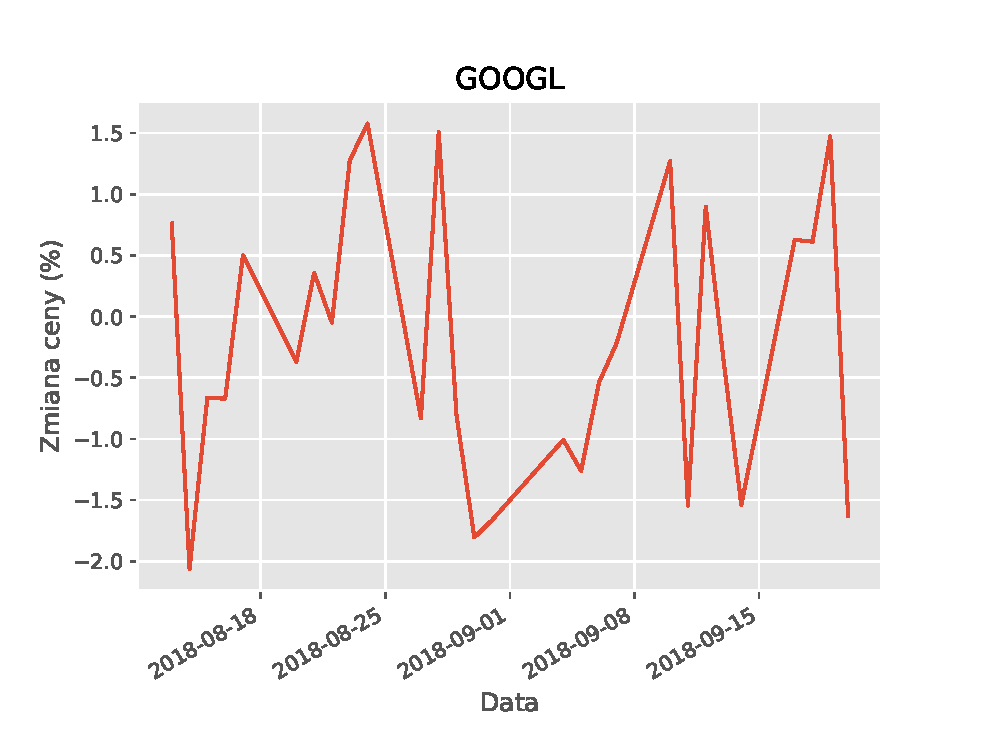
\includegraphics[scale=0.9]{img/linear_regression/l_r_pct_change_last_30}
\caption{Dzeinna zmiana ceny akcji spółki \textit{GOOGL} z 30 dni}
\label{l_r_pct_change_last_30}
\end{figure}


\subsubsection{Liczba dni}

Model przewidujący może na wyjściu przyjąć parametry z więcej niż jednego dnia sesji giełdowej. Należy uważać jednak na nakładanie się błędów predykcji i uważnie dobierać parametr przewidywanej ilości dni do przodu. Na przykład jeżeli prognozowana jest wartość z dwóch dni historii na trzy dni do przodu, to wówczas trzeci prognozowany dzień będzie oparty na prognozach dwóch poprzednich dni. W związku z czym dojdzie złączenia się błędu i mniej dokładnych wyników.

\subsubsection{Dobór danych pobranych z giełdy}

Według niektórych badań wolumen obrotów akcji nie jest skorelowany w żaden sposób z jej ceną. Modele mogą więc wykazywać lepsze wyniki przy mniejszej lub większej ilości danych wejściowych. Niektóre parametry mogą okazać się zbędne lub wręcz mogą osłabiać przewidywanie wartości.

\subsubsection{Dobór spółek uczących i testujących}

Modele oceniane na podstawie danych poszczególnych spółek mogą dawać w skrajnych przypadkach zafałszowane wyniki. Wiele spółek wykazuje wysoką korelację cen akcji między sobą. W celu uniknięcia pułapki przetrenowania, do uczenia i testowania użyte zostały dane spółek o niskiej korelacji i różnych trendach wzrostu/spadku.

\subsection{Ocena modeli}

Podczas oceny modelu wzięto pod uwagę różne kryteria mierzenia dokładności nauczonych klasyfikatorów.
\begin{itemize}
\item procent prawidłowych klasyfikacji
\item pole pod krzywą ROC
\item częściowy indeks Gini
\item statystyka H
\item współczynnik Briera
\item statystyka Kołomogrowa-Smirnova
\end{itemize}

\subsubsection{Procent prawidłowych klasyfikacji}

\subsubsection{Pole pod krzywą ROC}

\subsubsection{Częściowy indeks Gini}

\subsubsection{Statystyka H}

\subsubsection{Współczynnik Briera}

\subsubsection{Statystyka Kołomogrowa-Smirnova}

\section{Prognozowanie}

\subsection{Regresja liniowa}

Jedną z naiwnych metod przewidywania wartości funkcji jest regresja liniowa. Pierwszą próbą dla tego modelu było przewidzenie ceny zamknięcia z kolejnego dnia przy posiadaniu danych z dnia poprzedniego.

Z rysunku \ref{linear_regression_1} wynika iż prognozowane wartości pokrywają się z rzeczywistymi. Po obliczeniu błędu model daje nam dokładność na poziomie około  $99,934\%$. Wydaje się to być doskonałym wynikiem. Aby upewnić się o wartości modelu należy przyjrzeć się wykresowi z bliska.


\begin{figure}[H]%
\centering
\subfigure[Wykres rzeczywistych wartości]{%
\label{l_r_stock_data}
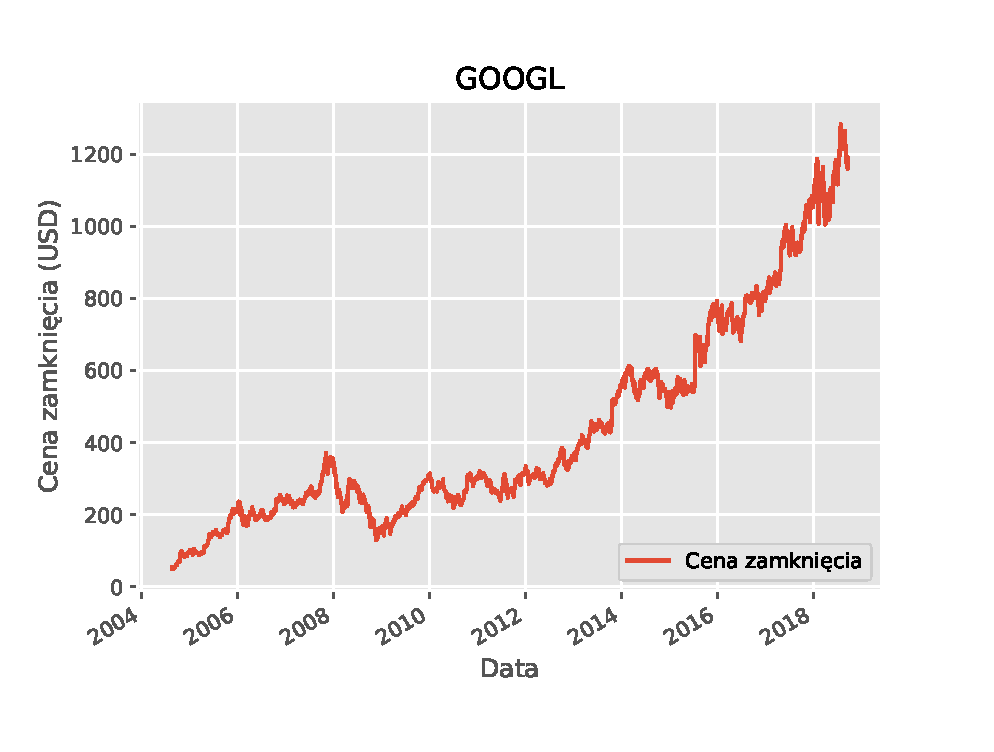
\includegraphics[scale=0.46]{img/linear_regression/l_r_stock_data}}%
\qquad
\subfigure[Wkyres rzeczywistych oraz przewidywanych wartości]{%
\label{l_r_1_day_full}
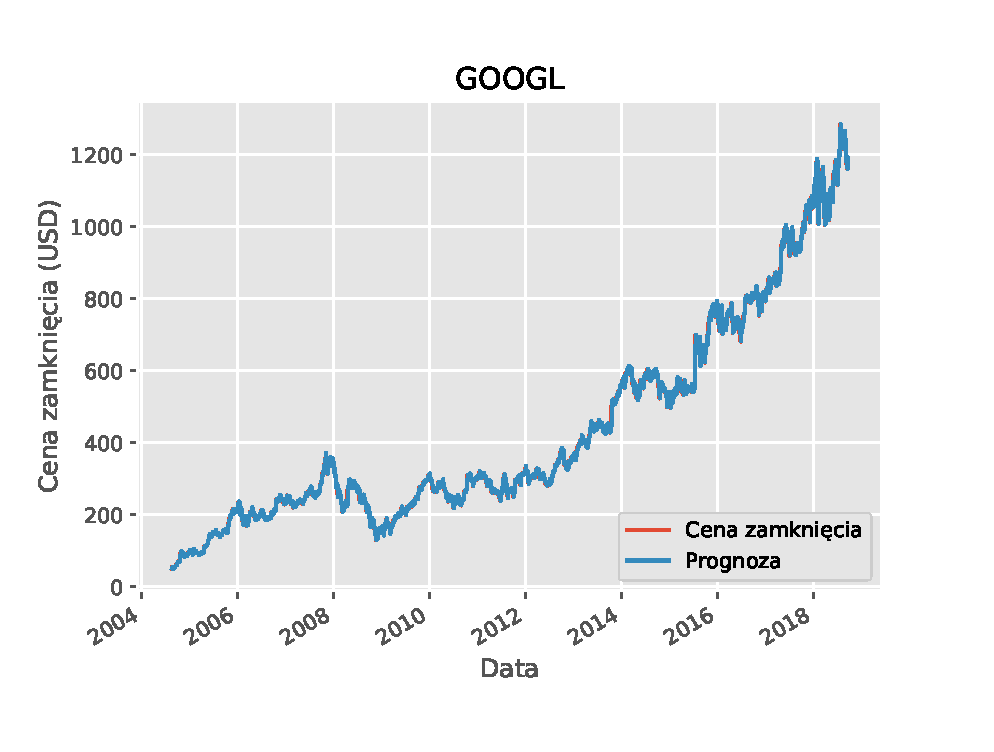
\includegraphics[scale=0.46]{img/linear_regression/l_r_1_day_full}}%
\caption{Wykres dla spółki \textit{GOOGL}}
\label{linear_regression_1}
\end{figure}


Na rysunku \ref{l_r_1_day_last_30} widać że prognozowane wartości są w rzeczywistości delikatnie zniekształconym obrazem przeszłych notowań spółki. Dokładność na poziomie $~99\%$ została osiągnięta ze względu na małe wahania w cenie. Logicznie rzecz biorąc nie jest to dobra metoda przewidywania przyszłości. Gdy cena jest w lokalnym maksimum wówczas inwestor powinien sprzedać posiadane akcje, jednak model przewiduje dalsze wzrosty ceny i wprowadza inwestora w błąd. Analogiczna sytuacja dzieje się przy minimach lokalnych ceny akcji. 

\begin{figure}[H]
\centering 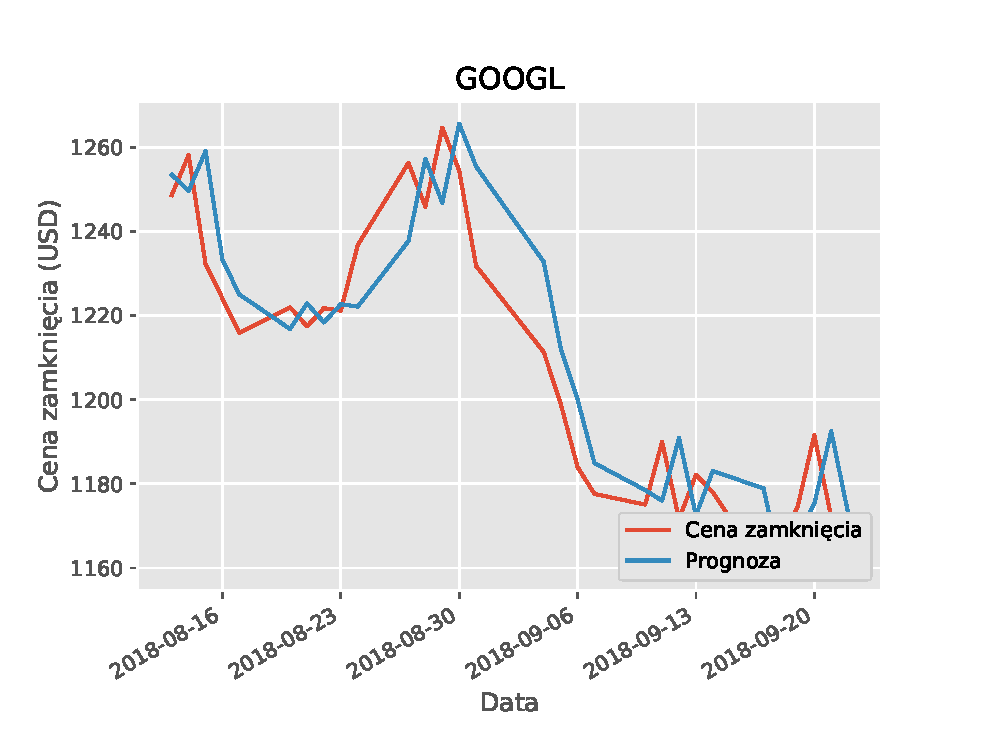
\includegraphics[scale=0.9]{img/linear_regression/l_r_1_day_last_30}
\caption{Wykres dla spólki \textit{GOOGL} z 30 dni}
\label{l_r_1_day_last_30}
\end{figure}


\bigskip

Wobec powyższych obserwacji należy sprawdzić jakość tego modelu w metodą dyskretnej. Dla tych samych prognoz została przeprowadzona ocena dyskretna z progiem $\pm0,4\%$. Na rysunku \ref{l_r_discrete_score} widoczna są przewidywane oraz rzeczywiste wartości oceny dyskretnej. Ze względu na charakterystyke regresji liniowej, niemal wszystkie prognozy oscylują w granicach, które są nieznaczące dla inwestora. Ocena tą metodą dała wynik $0.257\%$ co udowadnia bezużyteczność tego modelu. Dla porównania model losowy z rozkładem jednostajnym dałby wynik na poziomie $0.(3)\%$.


\begin{figure}[H]
\centering 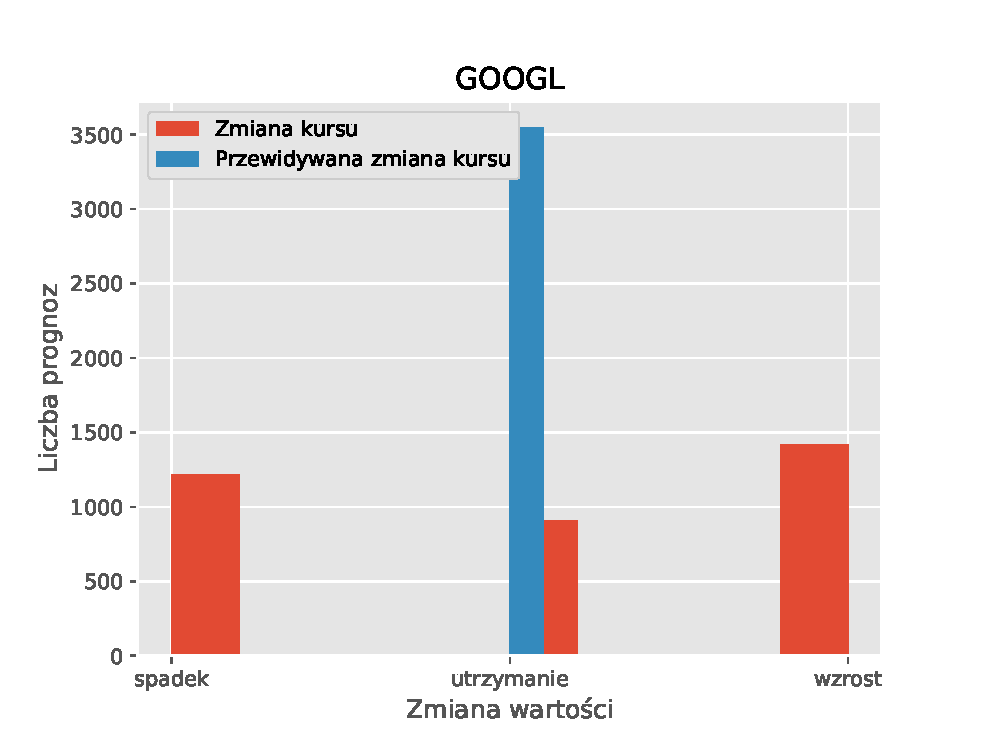
\includegraphics[scale=0.9]{img/linear_regression/l_r_discrete_score}
\caption{Histogram zmian cen akcji spółki \textit{GOOGL}}
\label{l_r_discrete_score}
\end{figure}

\subsection{Regresja logistyczna}

\subsection{SVM}

\subsection{Sieci neuronowe}

Sieci neuronowe są zbiorem modeli matematycznych służących do realizacji obliczeń, bądź przetwarzania sygnałów. Inspirowane działaniem mózgu, swoją nazwę czerpią z upodobnienia struktury do naturalnych neuronów oraz łączących je synaps. Głównymi zastosowaniami sieci neuronowych są zadania regresji, klasyfikacji oraz generowania danych.

\subsubsection{Sieci typu MLP}

Jednym z najprostszych przykładów sieci neuronowych jest perceptron wielowarstwowy (MPL). Taka sieć składa się z warstwy wejściowej, z dowolnej ilości warstw ukrytych oraz z warstwy wyjściowej. Na wejściu przyjmuje ona dane wejściowe, przetwarza dane i zwracają dane wyjściowe. Najprostszą implementacja sieci do predykcji danych giełdowych jest sieć przyjmująca na wejściu wektor informacji o akcjach spółki z jednego dnia, zwracająca na wyjściu przewidywaną wartość ceny akcji następnego dnia. Perceptron wielowarstwowy można również zaprojektować tak, aby na wyjściu zwracał wynik klasyfikacji, czyli procentowy wynik przypisania danych wejściowych do każdej z możliwych klas. W tej pracy badane były sieci neuronowe klasyfikujące dane wejściowe według trzech klas: spadek wartości poniżej pewnego progu, utrzymanie wartości w ramach tego progu oraz wzrost wartości powyżej tego progu. 

\subsubsection{Sieci rekurencyjne}

\subsection{GASEN}

\subsection{Sieć Bayesa}

\subsection{Średnia ważona zespołu klasyfikatorów}

\subsection{Wykorzystanie wykrywania sentymentu do poprawienia predykcji}

\section{Wspomaganie decyzji giełdowych}


\newpage

\renewcommand{\refname}{Bibliografia}
\begin{thebibliography}{9}
  
 \bibitem{nyse}
Strona główna NYSE
\\\url{https://www.nyse.com}
 
 \bibitem{nasdaq}
Strona główna NASDAQ
\\\url{https://www.nasdaq.com/}

 \bibitem{jpx}
Strona główna JPX
\\\url{https://www.jpx.co.jp/english/}

 \bibitem{alphavantage}
Strona główna Alpha Vantage
\\\url{https://www.alphavantage.co/}

 \bibitem{mongodb}
Strona główna MongoDB
\\\url{https://www.mongodb.com/}



\bibitem{randwalk}
  Burton G. Malkiel,
  \textit{Random Walk Down Wall Street: The Time-Tested Strategy for Successful Investing}.
  W. W. Norton Company,
  2007.

\bibitem{randwalk}
  John Hearty
  \textit{Advanced Machine Learning with Python}.
  Packt Publishing,
  2016.


\end{thebibliography}

\end{document}